\section{Characteristics of Exchange-Traded Funds}
\label{sec:ETFCharacteristics}
The creation and more recently the significant ownership share of Exchange-Traded Funds in major stock markets (among other asset classes) yields several empirical statements. For about a decade, further investigation has started measuring the impact of ETFs and confronting hypotheses while theory has been following with models that embed the mechanisms observed in practice :
\begin{itemize}
  \item how ETFs and mutual funds, as investment vehicles, can coexist in equilibrium, due to a trade-off between cost efficiency and exposure to liquidity shocks; more generally, the rise of ETFs coincides with debates about the effects of indexing (the rise of passive investment) and about the increasing concentration of institutional investors causing larger and more correlatied fund flows and subsequent comovements among securities.
\item how participants cause both the dry-up and increased price movements of multiple securities held through ETFs during high volatility times, a behavior that propagates turmoil in an unpredictable way;
  \item how ETFs may also increase pricing efficiency by providing arbitrageurs a proxy in order to sell short some securities that are precisely subject to short-sale limitations.
  \end{itemize}

These topics will be discussed in greater depth in the next section. First, in order to understand why ETFs have experienced such an outstanding growth\footnote{\dots whether measured in the number of products issued, the value of assets under management, the share in exchanged volume or the variety of asset classes, sectors and invesment styles covered\dots} and raised such concerns, it is necessary to describe how this structure appeals to investors and why they were a timely innovation that matched deep trends in financial markets' research and practice from the late \nth{20} century until now.
\subsection{Goal}
As it has been briefly exposed in the \nameref{Foreword}, ETF are the most successful implementation of an objective initially aimed at, and reached by, institutional investors. This objective was, then, to design a continuously, publicly tradable vehicle tracking a diversified value-weighted equity index. The first ETF issued on a U.S. exchange (back in 1993)  was indeed the SPDR S\&P 500 ETF, the archetype of the first products ever designed. Its net assets as of September 30, 2018, according to the trust prospectus, amount to nearly USD 280 billion, only USD 1.3 billion being held in cash. Several thousand products have appeared in the ETF category\footnote{At least 5400 ETFs were trading globally as of late 2017, according to research firm ETFGI. Source : \url{https://www.marketwatch.com/story/efts-shattered-their-growth-records-in-2017-2017-12-11}} as well as in the broader Exchange-Traded Products family. Assets under management amounted to more than USD 4.5 trillion. Although there are wide range investment objectives and sophisticated strategies, the fund with the highest absolute net inflows over the year (USD 30.2 billion) was the iShares Core S\&P 500 ETF.

\begin{figure}
    \centering
    \caption{Shift towards ETF investments and steady outflows from mutual fundsin U.S. equity}
    \label{fig:USFlows}
    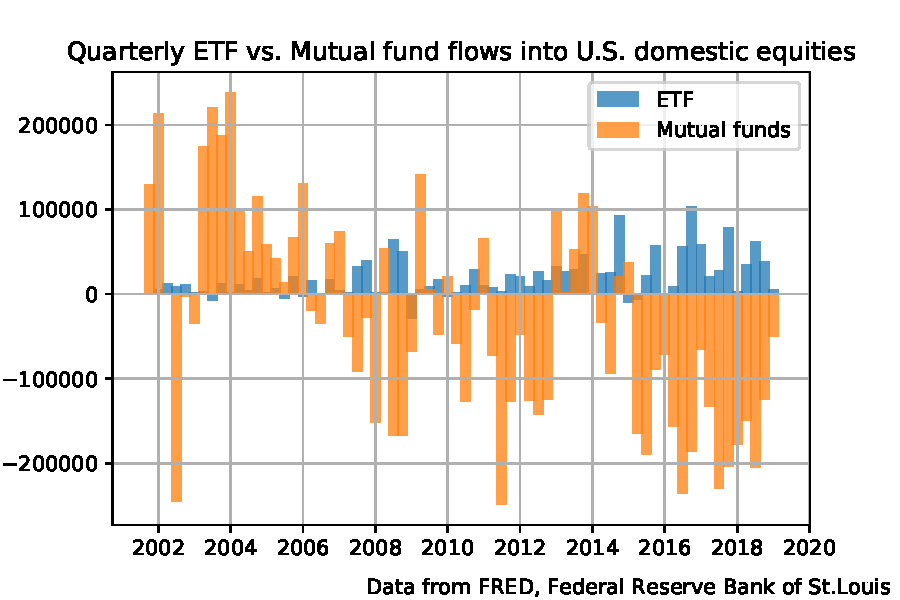
\includegraphics[width = \textwidth, height = 0.3\paperheight, keepaspectratio]{./Slides/USFlows_ETFvsMutual.pdf}
  \end{figure}

ETFs differ from open-end index funds, sometimes called \textit{traditional index funds}, in that they offer permanent liquidity throughout trading hours, they publish the fund's Net Asset Value at regular intervals and the creation/redemption of shares is the task of institutions entitled to exchange a basket of in kind securities for a newly created batch of ETF shares or to do the opposite trade with the fund sponsor to redeem ETF shares. The close tracking of the index is made possible by the privilege that authorized participants (APs), a designation essentially applied to market makers and brokers, enjoy to perform an arbitrage between the NAV and the actual value of underlying securities on the exchange. \parencite{Ben-David2017}

Standardized blocks of shares created and redeemed by ETF sponsors are called \emph{creation units}. In exchange for a basket of securities matching the current index composition and an amount in cash amounting to the value of dividends granted on stocks, the counterparty will receive a multiple of a fixed number of shares, e.g. $50000$ shares. The same process exists for in-kind redemption : in this case, the ETF hands back the basket of securities and erases a multiple of a creation unit. Actual delivery delays of assets vary according to regulation, allowing settlment within two trading days after the transaction date. In some situations, when participants can prove their failure to deliver is involuntary\footnote{The exact wording is :``their failure to deliver is the result of bona fide market making''. \parencite{Ben-David2017}}, trades may even be settled within three additional days. In U.S.-incorporated ETF markets, there is a clearinghouse processing transactions between authorized participants on one side and ETF issuers or their distributors on the other side; its name is the National Securities Clearing Corporation and it already was the major post-trade actor before ETFs existed. Once creations and redemptions are processed after the market close, the NSCC shares a portfolio composition file with all active corporations, based on information provided by the issuer. This file then serves as the list of securities and their relevant quantity that participants have to provide in order to receive a creation unit.

The primary market for creation units is an essential feature and it is considered by research as the channel allowing for shock transmission between ETFs and securities as well as between stocks that are commonly held. Commonality in liquidity is seriously supposed to araise because of the creation/redemption mechanism as will be discussed later in this paper.

\subsection{Market participants}
So far, two essential actors of the primary market have been mentioned :
\begin{description}
\item[the ETF sponsor, or issuer] is the firm managing the fund, whose name is attached to the product because it decides which benchmark the ETF tracks and how the replication strategy is implemented. Although portfolio weights are public information, trading schemes may stay confidential, because investor fees depend the implementation. If the index is computed by a third party, the sponsor will benefit from tracking a well-known index since the demand exhibits a preference for widely used broad-based or sector-based indices. Replicating an index provided through another specialized company (for instance S\&P, MSCI) comes at a cost, the license fee, which typically amounts to several basis points per year. The issuer is in charge of the SEC filing in the United States, before compliant documentation is published. They also appoint participants presented in this subsection.
\item[authorized participants (APs)] are essential because they initiate share creations and redemptions with the fund, based on a formal agreement with the fund. One has to recall that the price of an ETF is not automatically and instantly determined by the value of the index; nor is it derived from the last known value of its assets, the NAV. Rather, ETFs are securities traded on an exchange as their name says, which mean their price stems from supply and demand. Therefore the market price of ETF shares may deviate from the underlying index; unlike closed-end funds, ETFs are known for the scheme allowing to correct this deviation. Precisely, APs' non-mandatory role is to adjust the supply of ETF shares by providing either securities portfolios corresponding to the track index in order to create new blocks of ETF shares (excess demand of ETF shares) or handing back blocks, the creation units, to the issuer in order to get in-kind reimbursement in the form of underlying securities (excess supply of ETF shares). They are not paid by ETF sponsors, not constrained to be constantly monitoring the net asset value (NAV) either: actually, authorized participants have to pay the sponsor a creation fee (which may be fixed, independent from traded value). Their incentive is the same as market makers, and some institutions may play several roles on an ETF market : they will engage in a creation process if demand for is in excess. In other terms, they will execute a profitable trade by being able to sell the created units above the NAV, regularly disseminated by the sponsor. Of course, such an arbitrage only takes place if the trade's costs, including transaction fees on individual stocks and ETF creation fees, do not offset the profit earned on the difference between the ETF price and its intraday NAV. Thus, authorized participants generally are large banks, broker-dealers and market makers.
\end{description}

\clearpage
\section{Chronological background}
\label{sec:Chronology}
If one wants to understand how fundamental the shift to passive investment and ETFs is, it seems necessary to step back at least to the 1970s. Masses of workers in Western countries have accessed the financial markets during the strong post-war economic boom. Mutual funds were not invented in the second half of \nth{20} century, rather were they formally regulated as collective investment schemes in the 1930s and more generally as investment companies with the 1940 Act in the U.S. Traces of the earliest closed-end funds are said to have been found in the Netherlands, first in 1774 in the form of a merchant's investment trust and then after the Congress of Vienna at the Dutch king's initiative. The scheme has then spread in Europe including Switzerland among early financial places with a 1849-established company called \emph{Société civile genevoise d'emploi de fonds}. Modern open-end funds though more relevantly have a famous and long-lived ancestor with the \emph{Wellington Fund}, established 1928. This company from Pennsylvania was famously led by the late Jack Bogle, before he founded \emph{The Vanguard Group} which nowadays manages the Wellington fund. 

The trend of institutionalization of investment really took on after World War II and mutual funds gained a significant attraction power in the 1980s. Mutual funds have claimed to provide a performance relative to benchmarks that are reference indices, for example the market-capitalization-weighted stock index. On the other hand, as a consequence, passive investing has become more easily available for small, individual investors thanks to a new type of open-end mutual fund : the index fund, first (successfully) implemented by Jack Bogle. ETFs appeared more than a decade later\footnote{\textcite{Charupat2013} reports as common knowledge that the first ETF listed was the Toronto Stock Exchange Index Participation Units, a product that tracked the market-capitalization-weighted TSE 35 stock index. The ETF was launched in March 1990 and was replaced in 2000 with the iShares S\&P/TSX 60 Index Fund as the benchmark on the Canadian stock market was changed.} and remained confidential as long as the trust into mutual funds was untouched. The narrative according to which fund managers only work with their shareholder's sole interest in mind suffered increasing doubt due to public scandals : in 2003, several dozen companies were found by regulators to have violated multiple customer diligence rules, being accused of late trading and market timing. Mutual fund prices, unlike ETFs, are computed once a day at close; late trading by informed traders allowed them to trade at the set price during the stock market ``after-hours'', instead of having to wait for the next session's fund price. Such certain profit opportunity is considered an unfair advantage granted by the fund to some traders, as is the market timing charge. Mutual funds investors, again unlike ETF investors, are generally prevented to trade back and forth beyond a certain frequency for cost reasons, since the processing of orders induces costs borne by all fund investors, and for cash management reasons too, since the cash balance needed to face frequent and potentially massive selling orders is larger. Violating their own rules, some funds arbitrarily allowed some privileged investors engage in market timing. The aim of such fund managers was reportedly to boast larger assets, which in turn positively influence their own fees. Scandals and the increased focus on managers' actual value added in exchange for their advisory and management fees following the 2008 financial crisis did not abruptly stop mutual funds' growth but slowed it at the benefit of Exchange-Traded Funds, considered by many as the most liquid and transparent vehicles for passive and alternative investment.\autoref{fig:Chronological:ETFCapitalization} shows how ETF accounted for an increasing share of the worldwide stock market capitalization estimate, \autoref{fig:Chronological:ETFVolume} shows that their share in terms of trading volume outpaces their ownership. In other words, ETFs nowadays trade at a higher frequency, on average, that the rest of shareholders.

\begin{figure}
  \centering
  \caption{Market capitalization : total stock market versus ETFs}
  \label{fig:Chronological:ETFCapitalization}
  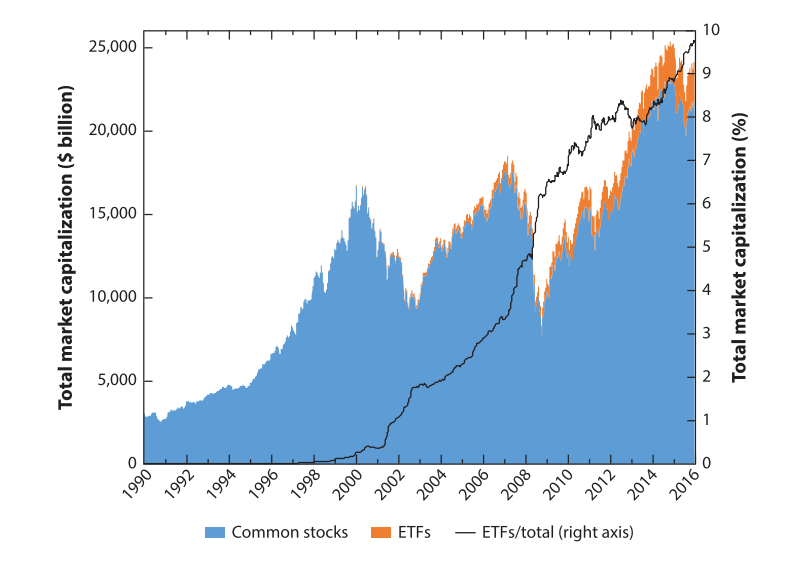
\includegraphics[width = \textwidth, height = 0.3\paperheight, keepaspectratio]{./Slides/Fig1_MarketCap}\\
  {\footnotesize Source: \textcite[172]{Ben-David2017}}
\end{figure}

\begin{figure}
  \centering
  \caption{Trading volume : total stock market versus ETFs}
  \label{fig:Chronological:ETFVolume}
  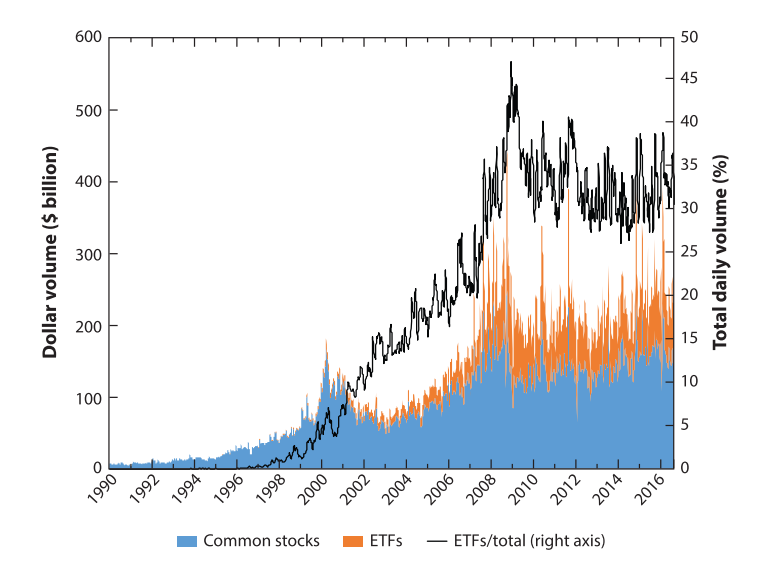
\includegraphics[width = \textwidth, height = 0.3\paperheight, keepaspectratio]{./Slides/Fig2_Volume}\\
  {\footnotesize Source: \textcite[173]{Ben-David2017}}
\end{figure}

The advent of Exchange-Traded Funds takes place in an ongoing debate that have led modern financial economics at least since Fama's paper about the Efficient Market Hypothesis (hereafter EMH) around 1965. The 2013 Nobel Prize granted to Eugene Fama \textit{and} Robert Shiller, EMH's main critic\footnote{As a matter of completeness, let us not forget the third recipient, Lars Peter Hansen, who developped econometric methods used to test the EMH, namely the General Method of Moments (GMM) estimators. A summary of their literature and the fields they contributed most to is \textcite{EconomicSciencesPrizeCommitteeoftheRoyalSwedishAcademyofSciences2012}} has obviously acknowledged the secular importance of the debate but the discussion has certainly not been closed since then.

In a recent working paper called \textit{The Active World of Passive Investing}, \textcite{Easley2018} claim that the shift from mutual funds and individual securities to ETFs is not simply a shift from active to passive investing, that distinction being ``antiquated''. Popular statistical metrics such as the active share -- which measures the absolute deviations of a portfolio holdings compared with a value-weighted benchmark -- and the tracking error -- i.e. the annualized standard deviation of the daily difference between the portfolio and market returns -- show that the decennial increase in ETFs share is actually fueled by active investing, including smart beta products whose ``activeness'' could be debated, because they essentially try to systematically capture risk premia justified by factors studied in the academic literature (most importantly, value and momentum factors). Nevertheless, a worldwide phenomenon has been at work leading to the mutual fund industry specializing towards passive investment and the ETF products, first designed to provide an efficient tracking of value-weighted stock indices, mutating to virtually any flavour of index, whether focusing on specific sizes, sectors, regions or factors.


In this paper, the focus is less on the mildly active aspect of ETF investing than on those products' impact on underlying assets. When agents shift from discretionary investing to index-tracking, the measure of success shifts from outperforming a benchmark to minimizing the difference between one's portfolio and a benchmark, and ETFs have shown that they are convenient instruments for this latter goal. It has been said that, with the variety of products available, the actual decision is not to pick the right security but the right index. Such change is suspected to induce some correlation among securities, a claim that this paper will address after a summary of related research.

\clearpage
\section{Review of literature}
\label{sec:Literature}
Different segments of research are relevant to this paper's questions, most of them, perhaps surprisingly, not considering ETFs specifically but studying the effects of indexing, derivatives, and institutional ownership.

Regarding the covariance of individual stock returns, a significant and positive impact of the contemporaneous share held by ETFs has been documented in several studies. An extensive \emph{Journal of Finance} article that inspires this paper, \textcite{Ben-David2018}, brings consistent evidence of this impact by analyzing the shock propagation through arbitrage between underlying securities and funds, using a sample of U.S. stocks and ETFs. First of all, they show that ETF on average exhibit higher liquidity (measured in the form of a lower \textcite{Amihud2002} \emph{illiquidity} ratio), a lower bid-ask spread and a higher turnover than the value-weighted baskets of securities they hold. This comparison method prevents an adverse selection bias due to ETF supposedly investing in the most liquid stock and being otherwise similar to their portfolio. This comparison is valid under the hypothesis that ETFs together hold a value-weighted basket of stocks, according to the traditional (and significant) use of ETFs.

Higher liquidity and turnover at the same time support the assumption of a clientele effect : as \textcite{Amihud1986} predicted in general and tested for NYSE stocks, investors with a shorter expected holding horizon have a preference for liquid securities and the relative bid-ask spread is a measure correlated with illiquidity. The focus on short term drives the investor's choice towards the most liquid stocks while buy-and-hold investors accept keeping less liquid assets since they do not expect and/or need to sell them immediately. 

\textcite{Ben-David2018} call their main hypothesis regarding a positive impact of ETF ownership over underlying stocks the \emph{liquidity trading hypothesis}: volatility reflects the fact that the shocks occurring on asset prices are non-fundamental, i.e. not related with cash flows nor with any news about the company. Therefore, the price is expected to revert to its initial value, ceteris paribus, because the shock is purely driven by liquidity. This sort of shock propagation differs from a two alternative hypotheses:
\begin{description}
\item[the price-discovery hypothesis]: permanent, i.e. fundamental, price adjustment related to some news spreading among investors. More precisely, this alternative hypothesis predicts that fundamental changes happen in the ETFs \emph{before} they hit the concerned stocks themselves. Having shown that ETF trading have an impact on the prices of underlying assets, the tests try to assess whether the shocks due to ETF trading have a permanent (fundamentally driven) or temporary (liquidity-driven) impact. The acceleration in stock prices' response to fundamental news has been documented in theory and empirical results in \textcite{Andrei2015} : in their model, there is a positive quadratic relationship between the time-varying degree of attention of investors and the stock's return variance, as well as a similar relation between learning uncertainty and variance, though weakly significant. This may come from the model, which specifies uncertainty as depending negatively from attention :  participants will learn more information by being more attentive and therefore reduce their uncertainty. In other terms, stable prices require the market to take news into account (attention) as well as converging to similar conclusions based on news (the opposite of uncertainty, i.e. trust in your forecasts). It is perhaps more intuitive to think of attention and uncertainty in terms of the proxy used empirically than based on the stochastic processes defined in the model : time-varying attention to news is proxied using statistics of Google searches on a financial and economic set of words, whereas uncertainty is derivded from the dispersion in analyst forecasts.
  \item[the liquidity buffer hypothesis]: instead of acting as a propagation channel for demannde shocks, ETF are supposed to act as substitutes for the underlying, less liquid securities since investors find the properties of stocks replicated in another liquid product. Thus, the introduction of an ETF captures part of the stocks's volatility non-fundamental volatility, which in turn decreases. This hypothesis was not developped in an ETF setting as it was first appeared in a commodity production model (\textcite{Danthine1978}) relating the introduction of futures with stabilized spot prices thanks to the information futures convey about rational expectations and therefore on supply -- although it is recognized that futures attracts speculators too. In short, this theory is used as if ETFs were the new futures and as if they could reflect expectations on the underlying assets. Empirical evidence with futures and stocks is not unanimous and results are mixed : the introduction of futures has been linked with an increase in the volatility of Nikkei index stocks. What is more, if one assumes that the futures market's importance is proxied through traded volume and open interest, \textcite{Bessembinder1992} find that indeed the introduction of futures decreased volumes exchanged on spot equity markets, that futures expected volume, resp. open interest, and spot volatility are negatively correlated together thanks to the increased market depth brought by futures. On the other side, the unexpected component of futures trading volume correlates positively with spot volatility. In general, their results are consistent with the hypothesis of the index arbitrage activity improving market depth highlighted in \textcite{Grossman1988} and they show no sign of support for increased instability due to liquid and relatively cheap correlated assets -- at that time, futures, and nowadays ETFs ?  
\end{description}
